\section{On the number of types in nowhere dense graph classes}

In this section we prove \Cref{thm:vc-density} and \Cref{thm:vc-density-lower-bound}.
	These results provide bounds on the number of types in classes of graphs which are nowhere dense, 
	and stronger bounds for classes which have bounded expansion. 
A class of graphs $\CCC$ has \emph{bounded expansion}
	if there is a function $d\colon\N\rightarrow\N$ such that for all 
	$r\in \N$ and all $H\minor_rG$ with $G\in\CCC$, the edge density
	of $H$, $|E(H)|/|V(H)|$, is bounded by $d(r)$. Note that every 
	class of bounded expansion is nowhere dense.
	
Throughout this section, fix a formula  $\phi(\tup x,\tup y)$, where
$\tup x$ is an $m$-tuple and $\tup y$ is an $n$-tuple of variables.

For a graph $G$, a set of  vertices $A\subset V(G)$, and a tuple $\tup v\in V(G)^n$,
denote
\[\phi(A,\tup v)=\setof{\tup a \in A^m }{ G\models\phi(\tup a,\tup v)}.\]
We call $\phi(A,\tup v)$ the \emph{$\phi$-type} of $\tup v$ \emph{over} $A$, and
$A$ is sometimes called the \emph{parameter set}.
For $W\subset V(G)$, denote
\[S_\phi(A,W)=\setof{\phi(A,\tup v)}{ \tup v\in W^n}.\]
Note that $S_\phi(A,W)$ is \emph{not} symmetric in $A$ and $W$.
We write $S_\phi(A,G)$ as a shorthand for $S_\phi(A,V(G))$. 
The set $S_\phi(A,G)$ is therefore the set of all $\phi$-types of $n$-tuples 
of vertices of $G$ over the parameter set $A$.

Our goal is to prove that if $G\in \CCC$, where $\CCC$ is a nowhere dense class,
then for every $\varepsilon>0$,   $|S_\phi(A,G)|\le \Oof(|A|^{n+\varepsilon})$, and 
$|S_\phi(A,G)|\le \Oof(|A|^n)$ if $\CCC$ is a class of bounded expansion.


First, observe that if $A\subseteq B$, then the number of types
over $A$ cannot be larger than the number of types over $B$. 

\begin{lemma}\label{lem:types-over-B}
Let $G$ be a graph and let $A\subseteq B\subseteq V(G)$. Then 
$|S_\phi(A,G)|\leq |S_\phi(B,G)|$. 
\end{lemma}

We will first enlarge the set $A$ to a set $B$, called
an \emph{$r$-closure of $A$}, such 
that the connections of elements from $V(G)\setminus B$ 
towards $B$ are well controlled. This approach
was first used in Drange et al.~\cite{drange2016kernelization} for
classes of bounded expansion and extended to nowhere dense
classes in Eickmeyer et al.~\cite{eickmeyer2016neighborhood}. 
Let us recall the necessary definitions.

Let $G$ be a graph and let $B\subseteq V(G)$ be a subset of vertices. For vertices $v\in B$ and $u\in V(G)\setminus B$, a path $P$ connecting $u$ and $v$ is called {\em{$B$-avoiding}}
if all its vertices apart from~$v$ do not belong to $B$. For a positive integer $r$ and $u\in V(G)\setminus B$, the {\em{$r$-projection}} of $u$ on $B$, denoted $M^G_r(u,B)$ is the set of all vertices $v\in B$ that
can be connected to $u$ by a $B$-avoiding path of length at most $r$. 
%
%The {\em{$r$-projection profile}} of a vertex $u\in V(G)\setminus A$ on $A$ is a function $\rho^G_r[u,A]$ mapping vertices of
%$A$ to $\{0,1,\ldots,r,\infty\}$, defined as follows: for every $v\in A$, the value $\rho^G_r[u,A](v)$ is the length of a shortest $A$-avoiding path connecting $u$ and~$v$, and~$\infty$ in case this length
%is larger than $r$. 
%
\begin{figure}[h!]
	\centering
		\includegraphics[scale=0.35,page=2]{pics}
	\caption{The  $r$-projection of $u$ on $B$
	(here $r=2$)
	is the minimal (inclusion-wise) set of $S\subset B$
	which $r$-separates $ u$ from $B$.
	}
	\label{fig:gaifman}
\end{figure}

We define 
\[\projnum_r(G,B)=|\{M_r^G(u,B)\colon u\in V(G)\setminus B\}|\]
%\quad\textrm{and}\quad \projprof_r(G,A)=|\{\rho_r^G[u,A]\colon %u\in V(G)\setminus A\}|\]
to be the number of different $r$-projections.
% and $r$-projection profiles realized on $B$, respectively. Clearly, it %holds that $\projnum_r(G,A)\leq \projprof_r(G,A)$.

\begin{lemma}[\cite{drange2016kernelization,eickmeyer2016neighborhood}]\label{lem:closure}
Let $\CCC$ be a class of graphs. 
\begin{enumerate}
\item If $\CCC$ has bounded expansion, then for every $r\in \N$ there is a constant $c\in \N$ such that for
every $G\in \CCC$ and $X\subseteq V(G)$ there exists a set $\cl_r(X)$, called an {\em{$r$-closure}} of $X$, with the following properties. 
\begin{itemize}
  \item $X\subseteq \cl_r(X)\subseteq V(G)$;
  \item $|\cl_r(X)|\leq c\cdot |X|$; and
  \item $|M_r^G(u,\cl_r(X))|\leq c$ for each $u\in V(G)\setminus \cl_r(X)$.
\end{itemize}
\item If $\CCC$ is nowhere dense, then for every $r\in\N$ and $\epsilon>0$ there is a 
constant $c\in\N$ such that for every $G\in \CCC$ and $X\subseteq V(G)$ there exists a set 
$\cl_r(X)$,  called an {\em{$r$-closure}} of $X$, 
with the following properties. 
\begin{itemize}
  \item $X\subseteq \cl_r(X)\subseteq V(G)$;
  \item $|\cl_r(X)|\leq c\cdot |X|^{1+\epsilon}$; and
  \item $|M_r^G(u,\cl_r(X))|\leq c\cdot |X|^{\epsilon}$ for each $u\in V(G)\setminus \cl_r(X)$.
\end{itemize}
\end{enumerate}
\end{lemma}

\begin{lemma}[\cite{drange2016kernelization,eickmeyer2016neighborhood}]\label{lem:projection-complexity}
Let $\CCC$ be a class of graphs. 
\begin{enumerate}
\item If $\CCC$ has bounded expansion, then for every $r\in \N$ there is 
  a constant $c\in\N$ such that for every graph $G\in \CCC$, and vertex subset $A\subseteq V(G)$, 
  it holds that $\projnum_r(G,A)\leq c\cdot |A|$.
  \item If $\CCC$ is nowhere dense, then for every $r\in \N$ and $\epsilon>0$ there is 
  a constant $c\in \N$ such that for every graph $G\in \CCC$, and vertex subset $A\subseteq V(G)$, 
  it holds that $\projnum_r(G,A)\leq c\cdot |A|^{1+\epsilon}$.
\end{enumerate}
\end{lemma}
Figure~\ref{fig:closure} summarizes the two lemmas 
in the nowhere dense case.

\begin{figure}[h!]
	\centering
		\includegraphics[scale=0.35,page=3]{pics}
	\caption{The  $r$-closure $B$ of $A$
has three properties:
(1) it's size is  $\Oof(|A|^{1+\epsilon})$,
(2) it has at most $\Oof(|B|^{1+\epsilon})$ distinct $r$-projections,
(3) every $r$-projection has size  $\Oof(|B|^\epsilon)$.
}
	\label{fig:closure}
\end{figure}

We informally sketch our proof of~\cref{thm:vc-density} in Figure~\ref{fig:sketch}.
\begin{figure}[h!]
	\centering
		\includegraphics[scale=0.35,page=4]{pics}
	\caption{Sketch of the proof of~\cref{thm:vc-density}. The precise values $\epsilon_1,\ldots,\epsilon_5$ need to be adapted suitably.
	%We rescale $\epsilon$	freely in the arguments.
	Fix $\phi$ of quantifier rank $q$ and let 
$r$ be the number obtained from~\cref{pro:crossing}.
Let $B$ be the $r$-closure of $A$. 
	Suppose that there are $|B|^{1+\epsilon_1}$ nodes with
	mutually distinct $\phi$-types over $B$.
	In the first step, we extract a set of $|B|^{\epsilon_3}$
	nodes which have the same $r$-projection $C$ to $B$;
	thus, they are $r$-separated from $B$ by $C$.
In the second step, using uniform quasi-wideness
with polynomial bounds,
	we further extract a subset of $|B|^{\epsilon_3/d}=|B|^{\epsilon_4}$ nodes
	(where $d$ is some constant)
	 which 
	are pairwise $2r$-separated by $S$, for some set of vertices $S$
	of constant size.
Since $|C|\le|B|^{\epsilon_2}$ 
it is easy to see that among these
	$|B|^{\epsilon_4}$ nodes,
there must be $|B|^{\epsilon_5}$
nodes which are $r$-separated from $B$ by $S$.
	Since $|S|$ is a constant,
	there is only a constant number of $(q,S)$-local types,
	so there must be two nodes $u,v$
	with the same $(q,S)$-local types, 
	which are $r$-separated from $B$ by $S$.
	By~\cref{pro:crossing}, $u$ and $v$ have the same types over $B$. This is a contradiction with the assumption the initial nodes $|B|^{1+\epsilon_1}$ had distinct $\phi$-types over $B$.	
	}
	\label{fig:sketch}
\end{figure}
For a formal proof, we formulate the following lemma,
which corresponds to the reasoning depicted in the figures caption,
starting from the point where a set of vertices with the same $r$-projection has been already selected.
\begin{lemma}\label{lem:num-types-same-class}
 Let $\CCC$ be a nowhere dense class,
let $G\in\CCC$ and let $B,C$ be sets of vertices with
$C\subset B\subseteq V(G)$.
Then, for any set of vertices $W\subset V(G)$ such that 
$M_r^G(v,B)\subseteq C$ for all $v\in W$, 
 $|S_\phi(B,W)|\le f(c)$, where $c=|C|$ and $f$ is a polynomial depending only on $\CCC$ and $\phi$.
\end{lemma}

\begin{proof}
Let $q$ be the quantifier rank of the formula $\phi$,
and let $r\in \N$ and~$T\from \N\times \N\times \N\to \N$  
be as described in~\cref{pro:crossing}.

Let $N^d\colon \N\times\N\to\N$ and $s^d\colon \N\to\N$ be
the functions for $\CCC$ described in \Cref{prop:uqw-tuples}. 
Let $s=s^n(2r)$, that is, we apply the function $s^d$ with
parameters $n$ and $2r$, and let $k\coloneqq T(q,n,s)$. In the parlance of~\cref{pro:crossing},
$k$ is a bound on the number of $(q,S)$-local types of vertices in a graph~$G$,
for any fixed $S\subset V(G)$ with $|S|\le s$. Recall that according
to \Cref{prop:uqw-tuples}, the function $N^d$ is polynomial in the second
argument. 

Let $Y\subseteq W^n$ be a maximal set of $n$-tuples 
such that $\phi(B,\tup u)\neq \phi(B,\tup v)$ 
for distinct $\tup u, \tup v\in Y$.
Suppose $|Y|\geq N^n(r,k+c+1)$. Then there is a  
set $S\subseteq V(G)$ of size $|S|\leq s$ 
and a set $X\subseteq Y$ of size $|X|\geq k+c+1$ which is 
mutually $2r$-independent in $G-S$. 
%\textcolor{red}{Furthermore, 
%on each coordinate that contains an element of $S$ we have 
%equality for all tuples. We now need a lemma that this is fine.} 

Consider the function $\pi\from V(G)\to P(C)$,
defined by the correspondence
 $v\mapsto M_r^{G-S}(v,B)$.
 Then, for distinct $\tup v,\tup w\in X$
 and $1\leq i,j\leq n$, 
 the sets $\pi(v_i)$ and $\pi(w_j)$ are pairwise disjoint subsets of $C$,
as otherwise we would have \mbox{$\dist_{G-S}(v_i,w_j)\leq 2r$},
contradicting mutual $2r$-independence.
As  $|X|\ge k+|C|+1$, it follows that 
there are at least $k+1$ tuples $\tup v\in X$
such that  $\pi(v)=\emptyset$ for every vertex $v$ appearing in $\bar v$. Let $Z$ denote the set of these tuples. Then the set of all those vertices appearing in~$Z$ and the
set $B$ are $r$-separated by~$S$.

Since $|Z|\geq k+1$ there are  distinct $\tup u,\tup v\in Z$ such that 
$\tup u$ and $\tup v$ have the same $(q,S)$-local types,
and from~\cref{pro:crossing}~\cref{c:confusing} it follows that $\tup u$ and $\tup v$
have the same quantifier rank $q$ type over $B$.
In particular, $\phi(B,\tup u)=\phi(B,\tup v)$. Since $\tup u,\tup v\in Y$, this contradicts the definition of $Y$. This proves $|Y|\le N^n(r,k+c+1)$,
and hence $|S_\phi(B,W)|=|Y|\le f(c)$ for 
$f(c)= N^n(r,k+c+1)$.
\end{proof}


Now, it is easy to conclude the main theorem. We repeat the statement of the theorem 
for convenience.

\setcounter{theorem}{2}
\begin{theorem}
Let $\CCC$ be a class of graphs and let $\psi(\tup x,y)$ be a first-order formula, where 
$\tup x$ is an $m$-tuple and $\tup y$ is an $n$-tuple of variables. 
\begin{enumerate}
\item If $\CCC$ is nowhere dense, then for every $\epsilon>0$ 
there exists a constant~$c$ such that for every $G\in \CCC$ and every
$A\subseteq V(G)$, we have $|S_\psi(A,G)|\leq c\cdot |A|^{n+\epsilon}.$

\item If $\CCC$ has bounded expansion, then there exists a constant~$c$ such that for every $G\in \CCC$ and every $A\subseteq V(G)$, we have $|S_\psi(A,G)|\leq c\cdot |A|^n$.
\end{enumerate}
\end{theorem}

\begin{proof}
We prove the statement about nowhere dense classes of graphs,
the bounded expansion case is proved analogously. 

Let $f$ be the polynomial from \Cref{lem:num-types-same-class},
depending on $\phi$ and $\CCC$. Assume $f(x)\leq c_0x^p$ 
for some constants $c_0$ and $p$. 
Choose $\epsilon'$ such that $(2n+p)\epsilon'+n\epsilon'^2=\epsilon$. 

Let $B$ be the closure of $A$ according to \Cref{lem:closure} with 
parameters $r$ and $\epsilon'$. According to the lemma, 
there is a constant $c_1$ such that 
we have $|M_r^G(u,B)|\leq c_1\cdot |A|^{\epsilon'}$ 
for each $u\in V(G)\setminus B$ and 
$|B|\leq c_1\cdot |A|^{1+\epsilon'}$. According to 
\Cref{lem:projection-complexity}, again applied
with parameters $r$ and $\epsilon'$, 
there is a constant
$c_2$ such that 
$\projnum_r(G,B)\leq c_2\cdot |B|^{1+\epsilon'}\leq
c_2\cdot (c_1\cdot |A|^{1+\epsilon'})^{1+\epsilon'}=c_1c_2\cdot|A|^{1+2\epsilon'+\epsilon'^2}$.
As $A\subseteq B$, 
according to \Cref{lem:types-over-B}, it suffices to bound the
number $|S_\phi(B,G)|$. 

We define an equivalence relation $\sim_r$ on 
$V(G)\setminus B$ by $u\sim_r v$ if 
$M_r^G(u,B)=M_r^G(v,B)$. 
Fix any $n$ equivalence
classes $\kappa_1,\ldots, \kappa_n$ (not necessarily
distinct) of $\sim_r$. Let $C=\bigcup_{1\leq i\leq n}M_r^G(u_i, B)$, 
where $u_i\in \kappa_i$ is any representative of the
equivalence class $\kappa_i$. Observe that $C\subseteq B$ with
$|C|\leq n\cdot c_1\cdot |A|^{\epsilon'}$. 
Then, according to \Cref{lem:num-types-same-class}, 
we have $|S_\phi(B,\bigcup_{1\leq i\leq n}\kappa_i)\leq
c_0\cdot |C|^p$. 

As we have at most $\mu_r(G,B)^n$ choices for 
$\kappa_1,\ldots, \kappa_n$, we count the total 
number of types as 
\begin{align*}
\mu_r(G,B)^n\cdot c_0\cdot |C|^p& \leq \left(c_1c_2|A|^{1+2\epsilon'+\epsilon'^2}\right)^n\cdot c_0\left(nc_1|A|^{\epsilon'}\right)^p\\
& =c_0c_1^{n+p}c_2^nn^p|A|^{n+(2n+p)\epsilon'+n\epsilon'^2}\eqqcolon c \cdot |A|^{n+\epsilon}.
\end{align*}

\end{proof}

\Cref{thm:vc-density-lower-bound}, which we also repeat for
convenience, is a simple consequence of the following two
lemmas. 

\begin{theorem}
Let $\CCC$ be a class of graphs which 
is closed under taking subgraphs. 
\begin{enumerate}
\item If $\CCC$ is somewhere dense, then there is a formula 
$\phi(x,y)$ such that for every $n\in \N$ there are $G\in\CCC$ and $A\subseteq V(G)$ 
with $|A|\geq n$ and $|S_\phi(A,G)|=2^{|A|}$. 
\item If $\CCC$ has unbounded expansion, then there is a formula 
$\phi(x,y)$ such that for every function $f:\N\rightarrow \N$ 
there are $G\in\CCC$ and $A\subseteq V(G)$ 
with $|S_\phi(A,G)|>f(|\phi|)\cdot |A|$. 
\end{enumerate}
\end{theorem}

Let $\mathcal{G}_r$ be the class of $r$-subdivisions of all 
simple graphs, that is, the class comprising
all the graphs that can be obtained from any simple graph by replacing every edge by a path of
length $r$.

\begin{lemma}[\cite{nevsetvril2011nowhere}]\label{lem:lower-nd}
For every somewhere dense graph class $\CCC$ that is closed 
under taking subgraphs, there
exists an integer $r_0$ such that $\mathcal{G}_{r_0}\subseteq \CCC$.
\end{lemma}

For $r\in \N$ and a graph $G$ denote by $\nu_r(G)$ the
\emph{$r$-neighborhood complexity} of $G$ as defined
by Reidl et al.~\cite{reidl2016characterising}, that is, the number 
\[\max_{H\subseteq G,\emptyset\neq X\subseteq V(G)}\frac{|\{N_r^H[v]\cap X : v\in V(H)\}|}{|X|}.\] 

A graph $H$ is a \emph{topological depth-$r$ minor} of $G$ if
there is a mapping $\phi$ that maps vertices of~$H$ to 
vertices of $G$ such that $\phi(u)\neq \phi(v)$ for 
$u\neq v$, and edges of $H$ to paths in 
$G$ such that if $uv\in E(H)$, then $\phi(uv)$
is a path of length at most $2r$ between $u$ and $v$ in 
$G$ and furthermore, if $uv, xy\in E(H)$, then 
$\phi(uv)$ and $\phi(xy)$ are internally vertex
disjoint. We write $H\minor_r^t G$. 
Note that the above definition makes sense for 
half-integers. 

\begin{lemma}[Theorem 4 of \cite{reidl2016characterising}]\label{lem:lower-be}
Let $G$ be a graph, let $r$ be a half-integer 
and let $H\minor_r^tG$. 
Then $|E(H)|/|V(H)|\leq (2r + 1)\cdot \max \left\{\nu_1(G)^4\cdot \log^2\nu_1(G),\nu_2(G),\ldots, \nu_{\left\lceil r+1/2\right\rceil}\right\}$.
\end{lemma}

\begin{proof}[of \Cref{thm:vc-density-lower-bound}]
To prove the first statement of \Cref{thm:vc-density-lower-bound}, 
for $n\in \N$, let $\PPP(n)$ denote the graph with $n+2^n$ 
vertices $V(\PPP(n))\coloneqq \{v_1,\ldots, v_n\}\cup \{w_M : M\subseteq \{1,\ldots, n\}\}$ and edges $E(\PPP(n))\coloneqq \{v_iw_M :1\leq i\leq n, M\subseteq \{1,\ldots, n\}, i\in M\}$. 
If $\CCC$ is somewhere dense and closed under taking subgraphs, 
according to \Cref{lem:lower-nd}, there exists an integer $r_0$ 
such that $\mathcal{G}_{r_0}\subseteq \CCC$, and in particular, 
$\{\PPP(n)_{r_0} :n\in \N\}\subseteq \CCC$. Now consider 
the formula $\phi(x,y)$ stating that $x$ and~$y$ have 
distance $r_0$. Then for every $n\in \N$ we have 
$S_\phi(\PPP(n),A)=2^{|A|}$, where $A\subseteq V(\PPP(n))$ denotes the set $\{v_1,\ldots, v_n\}$, which implies the statement
of the theorem.

For the second claim, we apply a result of Dvo\v{r}\'ak~\cite{dvorak2007asymptotical}, 
which relates the edge density of topological depth-$r$ minors
and depth-$r$ minors. In particular, the result of Dvo\v{r}\'ak
implies that a 
class $\CCC$ of graphs has unbounded expansion if and only 
if there is $r\in \N$ such that the value $|E(H)|/|V(H)|$ is unbounded
when $H$ ranges over all graphs such that $H\minor_r^tG $ for some $G\in \CCC$.
 By applying \Cref{lem:lower-be} and 
a standard Ramsey argument we find $r_0\leq r$ such that the value
$\nu_{r_0(H)}$ is unbounded when $H$ ranges over all graphs such that $H\minor_r^t G$
for some $G\in\CCC$. As above, consider 
the formula $\phi(x,y)$ stating that $x$ and~$y$ have 
distance $r_0$ to conclude. 
\end{proof}

